% Base numérica gerada de 20261011_historico_v3; narrativa revisada editorialmente.
% As tabelas foram preservadas. Regenerar este arquivo restaura a narrativa original.
% Ver Artigo/revisao_textual_manifest.json para a procedência desta revisão.
\subsection{Execução histórica ampliada}
\label{subsec:ampliacao-historica}

A coleta percorreu os 1.616 candidatos congelados, sem reposição. Foram registrados 29.088 cortes anuais, incluindo anos anteriores à existência do histórico: 17.087 sem snapshot, 11.850 com extração CK concluída, 62 sem fontes Java, 30 com erro de extração, cinco com inconsistências temporais e 54 com falha de recuperação. Os últimos correspondem aos 18 cortes de três repositórios indisponíveis, também verificados pelo identificador na API do GitHub. Um retorno 404 não permite distinguir remoção de mudança de visibilidade.

A confirmação do framework e os critérios por snapshot retiveram \textbf{388 projetos e 2.533 observações anuais}. São versões repetidas dos mesmos projetos, não 2.533 observações independentes. A Tabela~\ref{tab:historico-cobertura} informa a retenção por coorte. Os 116 candidatos antigos foram todos processados; 52 possuem ao menos uma versão elegível, somando 609 observações. As outras coortes oferecem contexto e não alteram esse conjunto principal.

A extração CK concluída não basta para tornar uma versão elegível: a comparação também exige confirmação do framework, porte mínimo e cobertura adequada. Por sua vez, um corte sem snapshot pode anteceder a existência do projeto, sem representar uma falha da ferramenta. Essas distinções impedem interpretar todos os registros fora da comparação principal como erros de coleta ou projetos de baixa qualidade.

\begin{table}[htbp]
\centering\small
\caption{Cobertura da execução histórica, por coorte de criação.}
\label{tab:historico-cobertura}
\begin{tabular}{lrrr}
\hline
Coorte & Candidatos & Projetos elegíveis & Snapshots elegíveis \\
\hline
E1 & 116 & 52 & 609 \\
E2 & 500 & 105 & 1.001 \\
E3 & 500 & 86 & 604 \\
E4 & 500 & 145 & 319 \\
Total & 1.616 & 388 & 2.533 \\
\hline
\end{tabular}
\end{table}

A auditoria automatizada validou a lista sorteada, os 18 registros por candidato, os limites temporais e as médias recalculadas dos dados brutos, incluindo produção e testes. Foram 3.142 extrações distintas, reutilizadas quando as fontes Java eram idênticas. A ampliação após o piloto consumiu aproximadamente 109 minutos com quatro trabalhadores, nas condições de cache da execução; clones e extrações ocuparam, respectivamente, 13,18 GiB e cerca de 598 MiB.

\paragraph{Emenda de classificação de framework.}
Um complemento de leitura de catálogos Gradle corrigiu 17 classificações anuais: dez no CAS e sete em RobotsJavaBackend. O complemento foi aplicado a toda a amostra, sem seleção pelo resultado CK. O segundo projeto permaneceu abaixo do tamanho mínimo; oito versões adicionais do CAS tornaram-se elegíveis e duas continuaram excluídas por submódulos não inspecionados. A classificação passou a reconhecer Boot no CAS desde 2016, após Spring tradicional em 2015, em vez de apenas em 2026. As métricas, os SHA, a amostra e as evidências de IA permaneceram idênticos nos 29.088 registros. Os manifestos conservam a emenda e a referência ao produtor CK original. Após a revisão da síntese para médias, os 88 testes passaram.

\subsection{Trajetórias dos projetos criados entre 2009 e 2013}
\label{subsec:trajetorias-antigas}

A Tabela~\ref{tab:historico-eras-e1} descreve exclusivamente a coorte antiga. Cada projeto contribui uma vez por época, pela média de seus snapshots elegíveis. E1 reúne 33 projetos e E4 reúne 43; esses conjuntos não são idênticos. Portanto, diferenças entre linhas combinam possíveis mudanças de código e de composição, não sendo uma comparação pareada dos mesmos projetos entre épocas.

\begin{table}[htbp]
\centering\scriptsize
\caption{Coorte antiga: médias por época do código, com produção e testes.}
\label{tab:historico-eras-e1}
\resizebox{\linewidth}{!}{\begin{tabular}{lrrrrrrrrr}
\hline
Época & Projetos & Snapshots & CBO & RFC & WMC & LOC/método & DIT & NOC & LCOM* \\
\hline
E1 & 33 & 71 & 5,758 & 8,111 & 8,781 & 5,985 & 1,346 & 0,201 & 0,289 \\
E2 & 43 & 155 & 5,934 & 8,552 & 9,155 & 6,127 & 1,329 & 0,161 & 0,295 \\
E3 & 47 & 168 & 6,068 & 8,525 & 8,889 & 6,252 & 1,344 & 0,177 & 0,295 \\
E4 & 43 & 172 & 6,238 & 8,838 & 9,029 & 6,173 & 1,317 & 0,173 & 0,289 \\
2026 parcial & 43 & 43 & 6,358 & 9,103 & 9,103 & 6,180 & 1,311 & 0,166 & 0,288 \\
\hline
\end{tabular}}
\end{table}

Entre E1 e E4, as médias passam pelos seguintes valores: CBO, de 5,758 para 6,238; RFC, de 8,111 para 8,838; WMC, de 8,781 para 9,029; LOC por método, de 5,985 para 6,173; DIT, de 1,346 para 1,317; NOC, de 0,201 para 0,173; LCOM*, de 0,2894 para 0,2890. Os indicadores variam em direções distintas. Esses valores não demonstram piora geral por haver aumentos, nem melhoria geral por haver reduções: tamanho, responsabilidades e composição dos projetos participam de sua interpretação.

A estabilidade também precisa ser interpretada: em 2025, 20 dos 43 snapshots elegíveis da coorte antiga repetem o SHA do corte anterior; em 2026, são 23 de 43. Assim, a distribuição inclui código legado mantido disponível, além de projetos em evolução ativa. A Figura~\ref{fig:historico-wmc} separa a média anual da amostra de contexto das trajetórias individuais antigas. Lacunas são conservadas nas tabelas; segmentos entre pontos não significam observações intermediárias.

\begin{figure}[htbp]
\centering
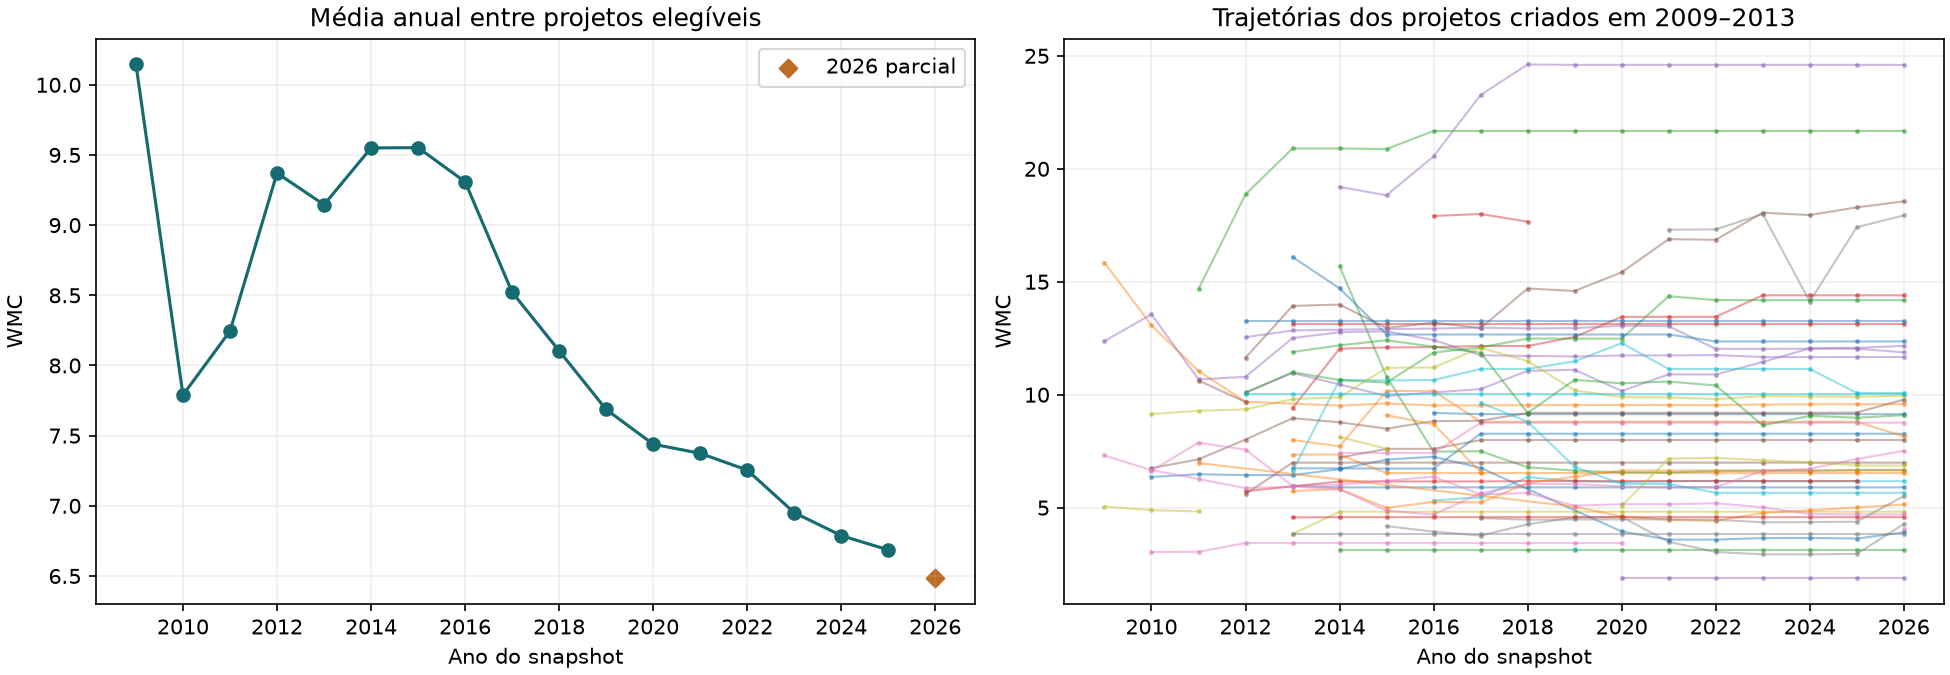
\includegraphics[width=\linewidth]{../Instrumentos/Codigos/Artefatos/evolucao_spring/runs/20261011_historico_v3/figures/avg_wmc.png}
\caption{WMC no histórico: média anual dos elegíveis de todas as coortes (esquerda) e trajetórias individuais da coorte antiga (direita). O período de 2026 é parcial. Mudanças da composição afetam as médias anuais.}
\label{fig:historico-wmc}
\end{figure}

\subsection{Mudanças que acompanharam Spring Boot}
\label{subsec:historico-boot}

Na coorte antiga, 16 projetos possuem versões elegíveis antes e depois da primeira presença anual observável de Boot, em anos completos. A Tabela~\ref{tab:historico-boot} mostra médias antes/depois e, separadamente, a média das diferenças calculadas projeto a projeto. Para os mesmos pares e pesos, a média das diferenças corresponde à média depois menos a média antes.

\begin{table}[htbp]
\centering\small
\caption{Spring Boot na coorte antiga: mesmos 16 projetos antes e depois ($n_a=n_b=16$).}
\label{tab:historico-boot}
\begin{tabular}{lrrr}
\hline
Métrica & Média antes & Média depois & Média das diferenças \\
\hline
CBO & 5,883 & 6,227 & 0,3447 \\
RFC & 9,277 & 9,490 & 0,2132 \\
WMC & 10,091 & 9,670 & -0,4208 \\
LOC/método & 6,257 & 6,203 & -0,0541 \\
DIT & 1,353 & 1,346 & -0,0069 \\
NOC & 0,103 & 0,102 & -0,0003 \\
LCOM* & 0,306 & 0,310 & 0,0043 \\
\hline
\end{tabular}
\end{table}

A média das mudanças é positiva para CBO, RFC e LCOM*, e negativa para WMC, LOC por método, DIT e NOC. As magnitudes descrevem esta amostra; não são testes de significância ou efeitos causais. Quatorze pares usam anos consecutivos, um tem intervalo de dois anos e o Causeway tem intervalo de oito anos entre versões elegíveis. Esse último agrega muitas mudanças concorrentes. No conjunto das quatro coortes, existem 21 pares completos de Boot. As tabelas de contexto preservam separadamente os projetos sem transição observada nas mesmas janelas.

A redução média de WMC descreve menor complexidade agregada por classe nos pares, mas não informa se a maioria dos projetos apresentou redução. De modo semelhante, o aumento médio de CBO não identifica quais dependências mudaram nem se eram necessárias às novas responsabilidades. Como não foi realizada uma análise específica da influência do par com oito anos de intervalo, não se afirma que a direção das médias permaneceria sem ele. Os grupos sem transição fornecem contexto descritivo, não um controle experimental equivalente.

Os casos já inspecionados ajudam a interpretar o marco observado: Hawtio passa de Spring tradicional em 2013 para presença de Boot em 2014, e BroadleafCommerce apresenta essa sequência entre 2016 e 2017. Esses intervalos localizam a mudança entre versões anuais, sem isolar uma migração de todas as demais alterações. Já o caso CAS mostra que a data reconhecida depende da capacidade do detector de resolver as declarações do build; uma configuração não reconhecida não comprova ausência anterior de Boot.

Também há Boot preliminar antes de 2014: o snapshot de 2013 de \texttt{spring-guides/gs-rest-service} declara 0.5.0.M6. Com 43 LOC, ele fica fora da comparação principal, mas permanece registrado. Isso não contradiz o lançamento estável de abril de 2014.

\subsection{Análise exploratória das evidências de IA}
\label{subsec:historico-ia}

Onze projetos antigos apresentam evidência em alguma versão elegível. Apenas um possui par em anos completos até 2025: OpenESPI-DataCustodian, de 2024 para 2025. A evidência de coautoria Claude foi integrada em 1º de julho de 2025; a data de autoria é 24 de junho. No mesmo ano aparece Boot, impedindo separar essas mudanças. CBO passa de 9,895 para 12,180 e WMC de 11,140 para 10,079. Esse caso isolado não representa o comportamento geral de projetos assistidos por IA.

Os outros dez pares antigos usam 2025 e o corte parcial de 2026, fixado em 11 de outubro de 2026 às 19:34:13 UTC. A Tabela~\ref{tab:historico-ia-parcial} mantém esse acompanhamento separado. Sinais como identidades de bot, arquivos de instruções e entradas de gitignore não determinam quanto código foi gerado nem demonstram uso contínuo.

No piloto, MyBatis/Spring apresentou uma identidade de bot Copilot, enquanto Hawtio apresentou um arquivo \texttt{AGENTS.md}. O primeiro sinal se refere à identidade registrada no histórico; o segundo, a instruções presentes no projeto. A reunião desses casos permite estudar a presença de vestígios, mas não estabelece uma exposição uniforme à assistência. Além disso, mudanças medidas entre o encerramento de 2025 e o corte parcial de 2026 podem anteceder a primeira evidência ou ocorrer depois dela dentro do mesmo intervalo.

\begin{table}[htbp]
\centering\small
\caption{IA na coorte antiga: dez pares com acompanhamento parcial em 2026 ($n_a=n_b=10$).}
\label{tab:historico-ia-parcial}
\begin{tabular}{lrrr}
\hline
Métrica & Média antes & Média parcial & Média das diferenças \\
\hline
CBO & 5,829 & 5,878 & 0,0489 \\
RFC & 9,460 & 9,958 & 0,4983 \\
WMC & 7,371 & 7,763 & 0,3913 \\
LOC/método & 6,924 & 6,994 & 0,0703 \\
DIT & 1,417 & 1,419 & 0,0020 \\
NOC & 0,159 & 0,139 & -0,0205 \\
LCOM* & 0,232 & 0,232 & 0,0006 \\
\hline
\end{tabular}
\end{table}

Na amostra de todas as coortes, há quatro pares de IA em anos completos e 17 pares adicionais no período parcial. As contagens são menores que o total de positivos porque nem todo projeto tem uma versão anterior elegível sem evidência. Esses resultados permitem descrever os casos, mas não sustentar uma conclusão geral de melhora ou piora associada à IA. A ausência dos sinais procurados também não estabelece um grupo comprovadamente sem uso.

\subsection{Interpretação conjunta}

O acompanhamento histórico mostra que permanência, mudança estrutural e adoção de ferramentas são fenômenos distintos. Um projeto pode repetir código por vários anos, incorporar Boot em um intervalo e apresentar vestígios de IA muito depois. O valor do desenho está em localizar essas observações em versões verificáveis, evitando atribuir uma tecnologia atual a toda a história do repositório.

As direções distintas das métricas não constituem um teste que refute o progresso da comunidade. Elas delimitam o que esta descrição permite afirmar sobre a amostra, diante de mudanças de composição e de contexto. A resolução anual e os indicadores Java também não capturam todas as alterações de configuração, funcionalidade ou esforço. As conclusões a seguir respondem às perguntas do estudo nesse alcance.
